\item \textbf{{[}ALVL/9597/2017/P2/Q3{]} }
\begin{enumerate}
\item Explain what is meant by an object in object-oriented programming.
.\hfill{}{[}2{]} 
\item {} 
\begin{enumerate}
\item A student is writing a program to represent people in a university.
Tutors, office workers, lecturers and professors are all employed
by the university. A professor is a senior lecturer. The university
educates both undergraduate and graduate students. 

The student\textquoteright s program contains a class with the identifier
\texttt{Person}. Sub-classes share the characteristics of this class. 

Copy and complete the following inheritance diagram by adding sub-classes
\texttt{Professor}, 

\texttt{OfficeWorker}, \texttt{Lecturer}, \texttt{Undergraduate},
\texttt{Staff}, \texttt{Graduate}, \texttt{Student} and \texttt{Tutor}.
\hfill{}{[}2{]} 
\begin{center}
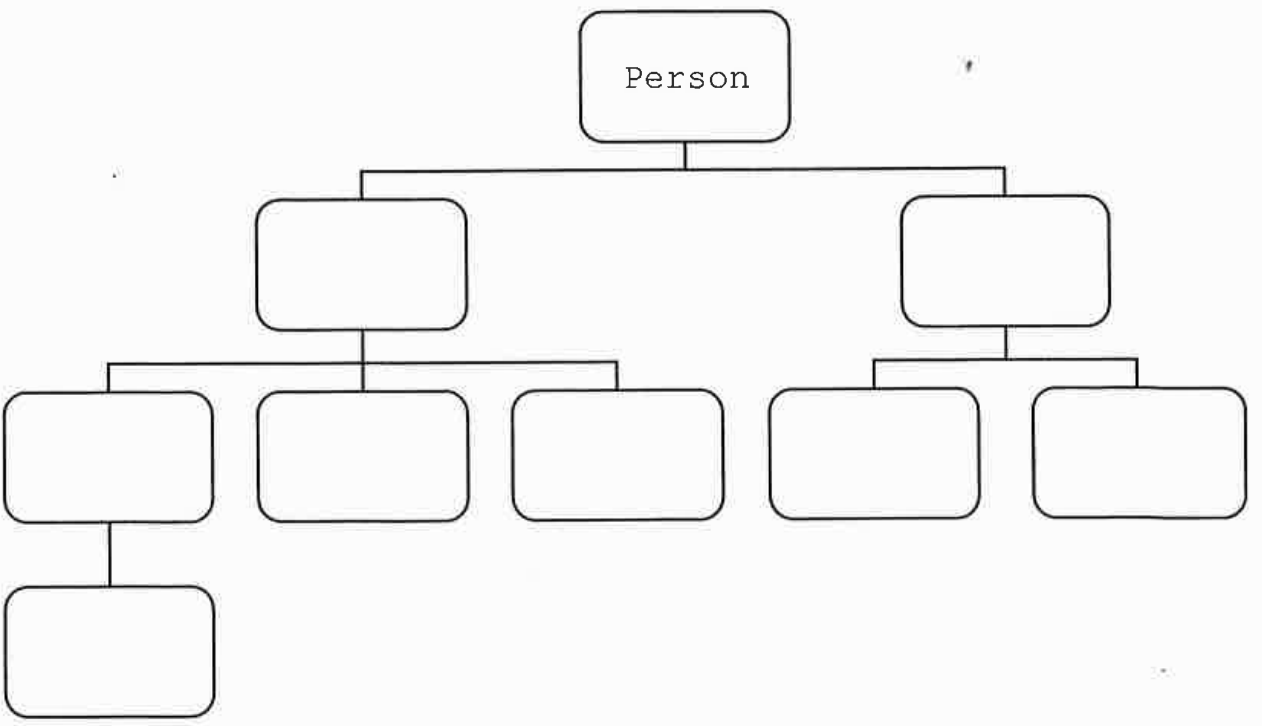
\includegraphics[width=0.5\paperwidth]{C:/Users/Admin/Desktop/Github/question_bank/LyX/static/img/9597-ALVL-2017-P2-Q3}
\par\end{center}
\item Explain why inheritance is an important feature of object-oriented
programming.\hfill{}{[}2{]} 
\end{enumerate}
\item A stack is a data structure that can be implemented in object-oriented
programming. The implementation of a stack requires an integer variable
and an array. 
\begin{enumerate}
\item Describe the purpose of the integer variable in the implementation
of a stack class.\hfill{} {[}1{]}
\item Describe the purpose of the array in the implementation of a stack
class.\hfill{} {[}1{]}
\item Explain how to use the stack data structure to compute the following
expression: 
\noindent \begin{center}
$\left(\text{A}+\text{B}\right)\times\left(\text{C}+\text{D}\right)$\hfill{}
{[}2{]}
\par\end{center}

\end{enumerate}
\end{enumerate}